%\documentclass[conference]{IEEEtran}
\documentclass[10pt,conference,anonymous]{IEEEtran}
\IEEEoverridecommandlockouts

%% Marcelo added this
\makeatletter
\renewcommand\footnoterule{%
  \kern-3\p@
  \hrule\@width.4\columnwidth
  \kern2.6\p@}
  \makeatother




\usepackage{inconsolata}
\usepackage{listings}

\lstset{language=Java,
basicstyle=\ttfamily\scriptsize,
%basicstyle=\ttfamily,
keywordstyle=\color{javapurple}\bfseries,
stringstyle=\color{pblue},
commentstyle=\color{javagreen},
morecomment=[s][\color{javadocblue}]{/**}{*/},
morecomment=[s][\color{gray}]{@}{\ },
numbers=left,
numberstyle=\tiny\color{black},
stepnumber=2,
numbersep=8pt,
tabsize=4,
showspaces=false,
showstringspaces=false,
breaklines=true,}

%%%%%%%%%%%%%%%%%%%%%%%%%%%%%%%%%%




\usepackage{adjustbox} % ajustar tabela ao tamanho da pagina

\usepackage{tikz}
\usetikzlibrary{matrix,fit,shapes,calc,positioning,shadows,arrows,shapes,backgrounds,decorations.markings,fadings}
\usepackage{graphicx}
\usepackage{multirow}
\usepackage[caption=false, font=footnotesize]{subfig}
\usepackage{wrapfig}
\usepackage{enumitem}
\usepackage{url}
%% helpers
\newcommand{\js}{JS}
\newcommand{\javascript}{JavaScript}
\newcommand{\es}{ES}
\newcommand{\ecmascript}{\es{}}
\newcommand{\tname}{TNAME}
\newcommand{\Comment}[1]{}
\newcommand{\numsubjects}{5}
\newcommand{\etal}{and colleagues'}
\newcommand{\ie}{i.e.}
\newcommand{\eg}{e.g.}
\newcommand{\cmark}{\ding{51}}%
\newcommand{\xmark}{{\color{red}\ding{55}}}%
\newcommand{\pGoodGood}{$\mathit{P}${\small\cmark\!\cmark}}%
\newcommand{\pGoodBad}{$\mathit{P}${\small\cmark\!\xmark}}%
\newcommand{\pBadDontCare}{$\mathit{P_?}$}%
\newcommand{\sfl}{SFL\xspace}
\newcommand{\ddg}{DDG\xspace}
\newcommand{\totfiles}{$\sim$38K}

%% annotations
\newif\ifdraftmode
%% Comment or uncomment the \draftmodetrue line.
\draftmodetrue
\ifdraftmode
 \newcommand{\Fix}[1]{\textbf{[[}{\color{red} #1}\textbf{]]}}
 \newcommand{\Mar}[1]{\textbf{[[Marcelo: }{\color{magenta} #1}\textbf{]]}}
 \newcommand{\Igor}[1]{\textbf{[[Igor: }{\color{blue} #1}\textbf{]]}}
 \newcommand{\note}[1]{\todo[inline,color=red!30,caption={}]{#1}}
\else
 \newcommand{\Fix}[1]{\relax}
 \newcommand{\Mar}[1]{\relax}
 \newcommand{\Igor}[1]{\relax}
 \newcommand{\note}[1]{\relax}
\fi

% For submitted version only.
\pagenumbering{arabic}

% Uncomment this if you need more space
%% \makeatletter
%% \def\@copyrightspace{\enlargethispage{-10pt}\relax}
%% \makeatother

\newcommand{\codesize}{\small}
\newcommand{\CodeIn}[1]{\mcodeid{#1}}
\newcommand{\CodeInM}[1]{\mcodeid{#1}}
% \|name| or \mathid{name} denotes identifiers and slots in formulas
\def\|#1|{\mathid{#1}}
\newcommand{\mathid}[1]{\ensuremath{\mathit{#1}}}
% \<name> or \codeid{name} denotes computer code identifiers
\def\<#1>{\codeid{#1}}
\newcommand{\codeid}[1]{\ifmmode{\mbox{\codesize\ttfamily{#1}}}\else{\codesize\ttfamily #1}\fi}
\def\<#1>{\mcodeid{#1}}
\newcommand{\mcodeid}[1]{\mbox{\codesize\ttfamily{#1}}}

%% thumbs up down
\newcommand*{\RightThumbsUpAux}[1]{%
  \begingroup
    \sbox0{Ag}%
    \raisebox{-\dp0}{%
      \includegraphics[{%
        height=\dimexpr\dp0+\ht0\relax,
        #1%
      }]{thumbsup.pdf}%
    }%
  \endgroup
}
\newcommand*{\RightThumbsUp}{%
  \RightThumbsUpAux{}%
}
\newcommand*{\RightThumbsDown}{%
  \RightThumbsUpAux{origin=c,angle=180}%
}
\newcommand*{\LeftThumbsUp}{%
  \scalebox{-1}[1]{\RightThumbsUp}%
}
\newcommand*{\LeftThumbsDown}{%
  \scalebox{-1}[1]{\RightThumbsDown}%
}

\newcommand{\checkm}{Y}
\newcommand{\crossmark}{N}
%\begin{wraptable}[20]{t}[0pt]{0.5\textwidth}

\newcommand{\totalTestFiles}{38,369}
\newcommand{\totalTestFilesCompileInAll}{35,939}
\newcommand{\totalTestFilesPassInAll}{24,493}
\newcommand{\nofuzzAll}{209}
\newcommand{\nofuzzBugs}{\Fix{XX}}
\newcommand{\nofuzzDuplicates}{63}
\newcommand{\nofuzzFalsePositives}{24}
\newcommand{\nofuzzHITotal}{177}
\newcommand{\nofuzzLOTotal}{32}
\newcommand{\nofuzzTotalFiles}{977} % conflicting files
\newcommand{\nofuzzFilesHI}{940} % conflicting files HI
\newcommand{\nofuzzFilesLO}{37} % conflicting files LO

\newcommand{\nofuzzBucketsBugsHI}{\Fix{124}} % buckets reported (including dups)
\newcommand{\nofuzzBucketsBugsLO}{\Fix{11}} % buckets reported
\newcommand{\nofuzzDupsHI}{\Fix{X}}
\newcommand{\nofuzzDupsLO}{\Fix{Y}}

% continue updating bugs table
\newcommand{\tableBugsNum}{\Fix{26}}

%% anonymize

\newcommand{\anonym}[1]{{\tiny\colorbox{black}{#1}}}

%% names
\newcommand{\radamsa}{radamsa}
\newcommand{\quickfuzz}{quickfuzz}

\newcommand{\jsc}{JavaScriptCore}
\newcommand{\veight}{V8}
\newcommand{\chakra}{Chakra}
\newcommand{\smonkey}{SpiderMonkey}
\newcommand{\jerry}{JerryScript}

\newcommand{\lo}{lo}
\newcommand{\hi}{hi}


\begin{document}

%Should I Fuzz my Inputs or Improve my Tests? 
\title{Lessons Learned from Differential Testing JS Engines}

%% \author{
%% \IEEEauthorblockN{Sabrina Souto}
%% \IEEEauthorblockA{State University of Para\'iba\\
%% Para\'iba, Brazil\\
%% sabrinadfs@gmail.com}
%% \and
%% \IEEEauthorblockN{Marcelo d'Amorim}
%% \IEEEauthorblockA{Federal University of Pernambuco\\
%%   Pernambuco, Brazil\\
%%   damorim@cin.ufpe.br}
%% \and
%% \IEEEauthorblockN{Rohit Gheyi}
%% \IEEEauthorblockA{Federal University of Campina Grande\\
%%   Para\'iba, Brazil\\
%%   rohit@dsc.ufcg.edu.br}
%% }

\maketitle

%% page numbering -M
\thispagestyle{plain}
\pagestyle{plain}

%% JavaScript (\js{}) is a popular programming language for the
%% web. Finding errors in JS runtime engines is an important problem.
\begin{abstract}
This paper assesses the impact of Differential Testing (DT) to find
functional bugs in JS engines. This is an important problem given the
importance of JS today. DT has shown successful in finding bugs in
compilers and runtimes, but has not been thoroughly explored in this
important domain. Our study \Fix{...}
\end{abstract}

\begin{IEEEkeywords}
...
\end{IEEEkeywords}

\section{Introduction}

JavaScript (\js{}) is today one of the most popular programming
languages for the web~\cite{business-insider,stackify}. The interest
of the community for the language encourages constant improvements in
its specification and implementations. It is natural to expect that
such improvements will entail sensible changes in runtime
engines~\cite{kangax}; changes that could lead to errors. Finding bugs
on JS engines is an important problem. In this paper, we are
particularly interested in finding functional (non-crash) bugs.

Differential testing~\cite{Brumley-etal-ss07} (DT) is a popular
approach that has been applied in a variety of contexts to find
functional
bugs~\cite{Yang-etal-pldi11,Chen-etal-fse2015,Argyros-etla-ccs16,Chen-etal-pldi16,petsios-etal-sp2017,SivakornAPKJ17}. DT
automates test generation in scenarios where multiple implementations
of a system exist. It leverages the diversity across system's
implementations to detect anomalous behavior. This paper reports the
results of a study we conducted to assess the impact of DT in finding
bugs on \js{} engines.


\Mar{this needs work$\rightarrow$} \Fix{but it has not been
  thoroughly explored to find functional bugs in JS engines. The
  closest work was done by Patra and Pradel~\cite{patra2016learning},
  where they evaluated their proposed language-agnostic fuzzer to find
  cross-browser HTML+JS discrepancies. This project aims at building
  and evaluating an infrastructure for differential testing of runtime
  engines, such as the JS engine or WebAssembly's. The sensible parts
  of the infrastructure are the checks of input validity (as to reduce
  waste/cost) and output correctness (as to reduce false positives).}

\section{Infrastructure}
\label{sec:design}


%\begin{wrapfigure}[10]{r}[0pt]{0.45\textwidth}
\begin{figure}[t]
  \centering
%  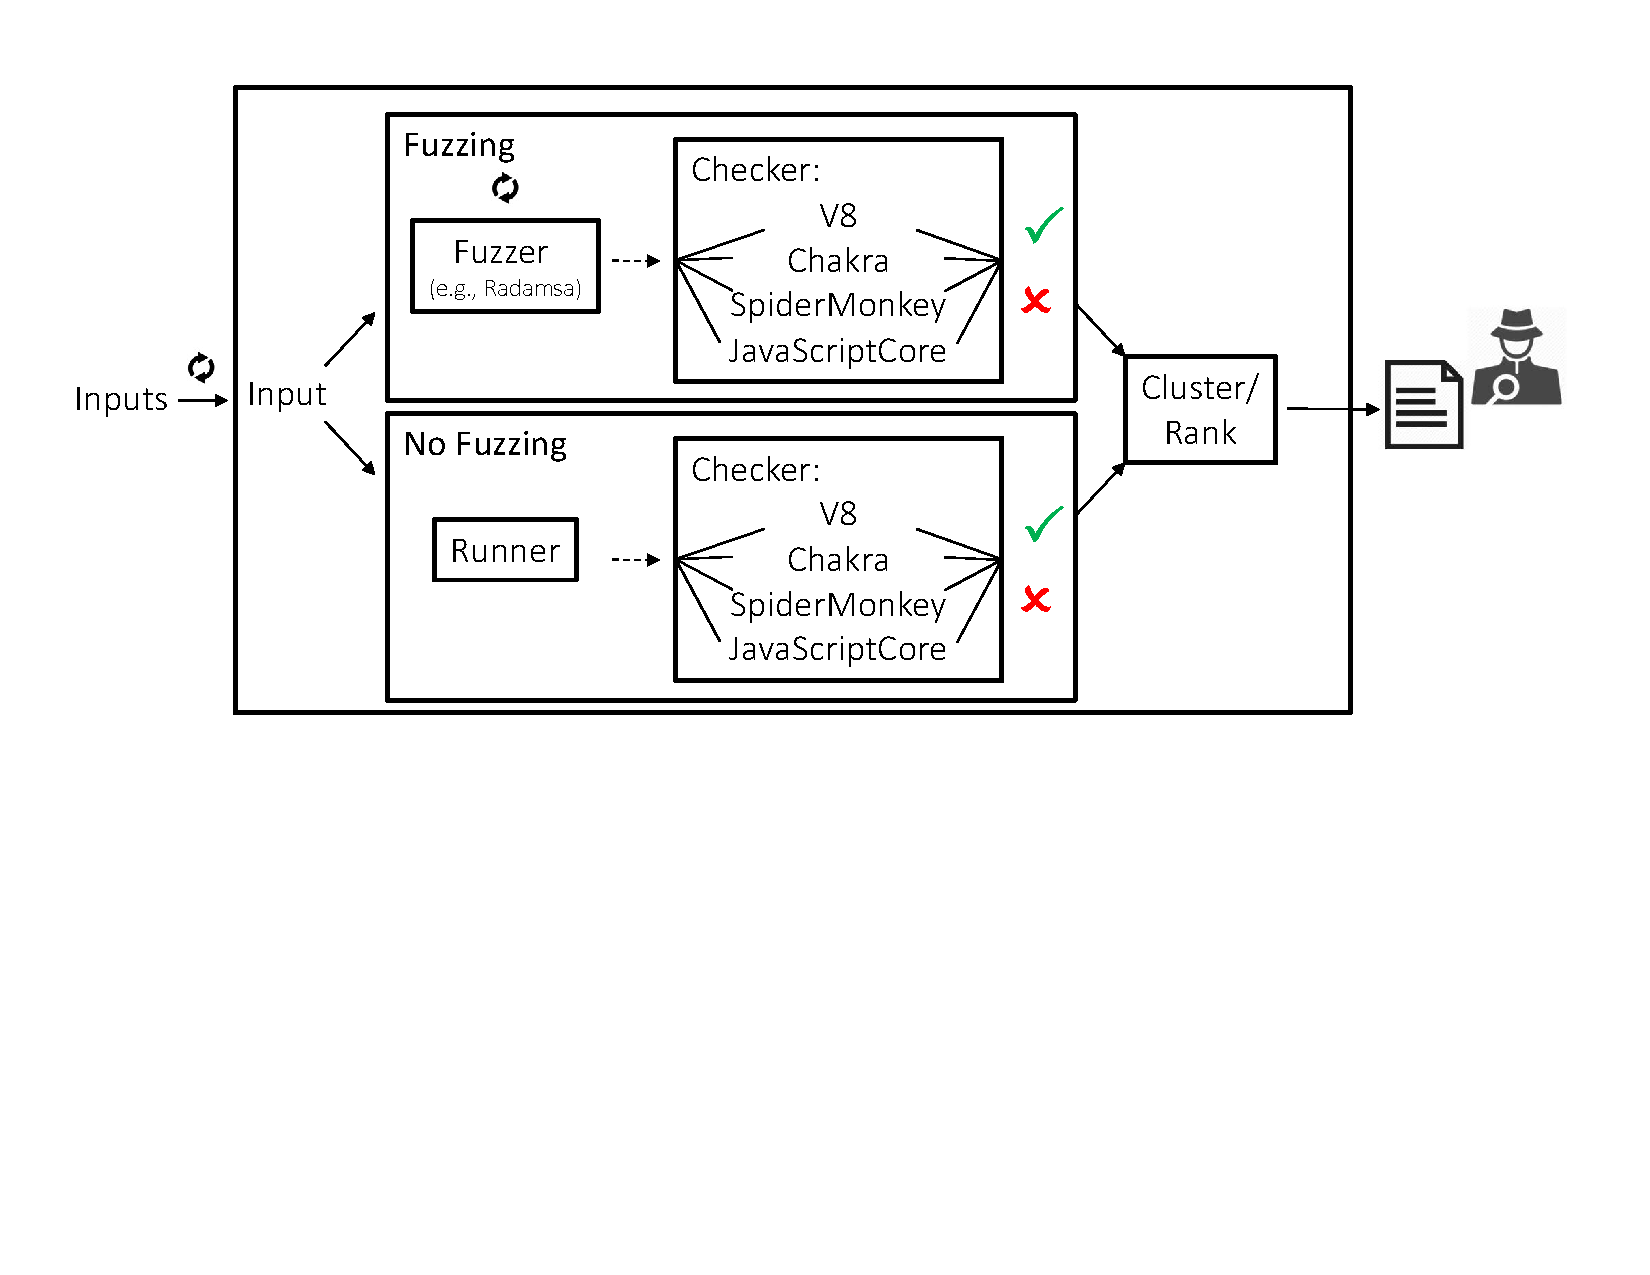
\includegraphics[trim=20 350 200
%    0,clip,width=0.35\textwidth]{google-awards-workflow}
  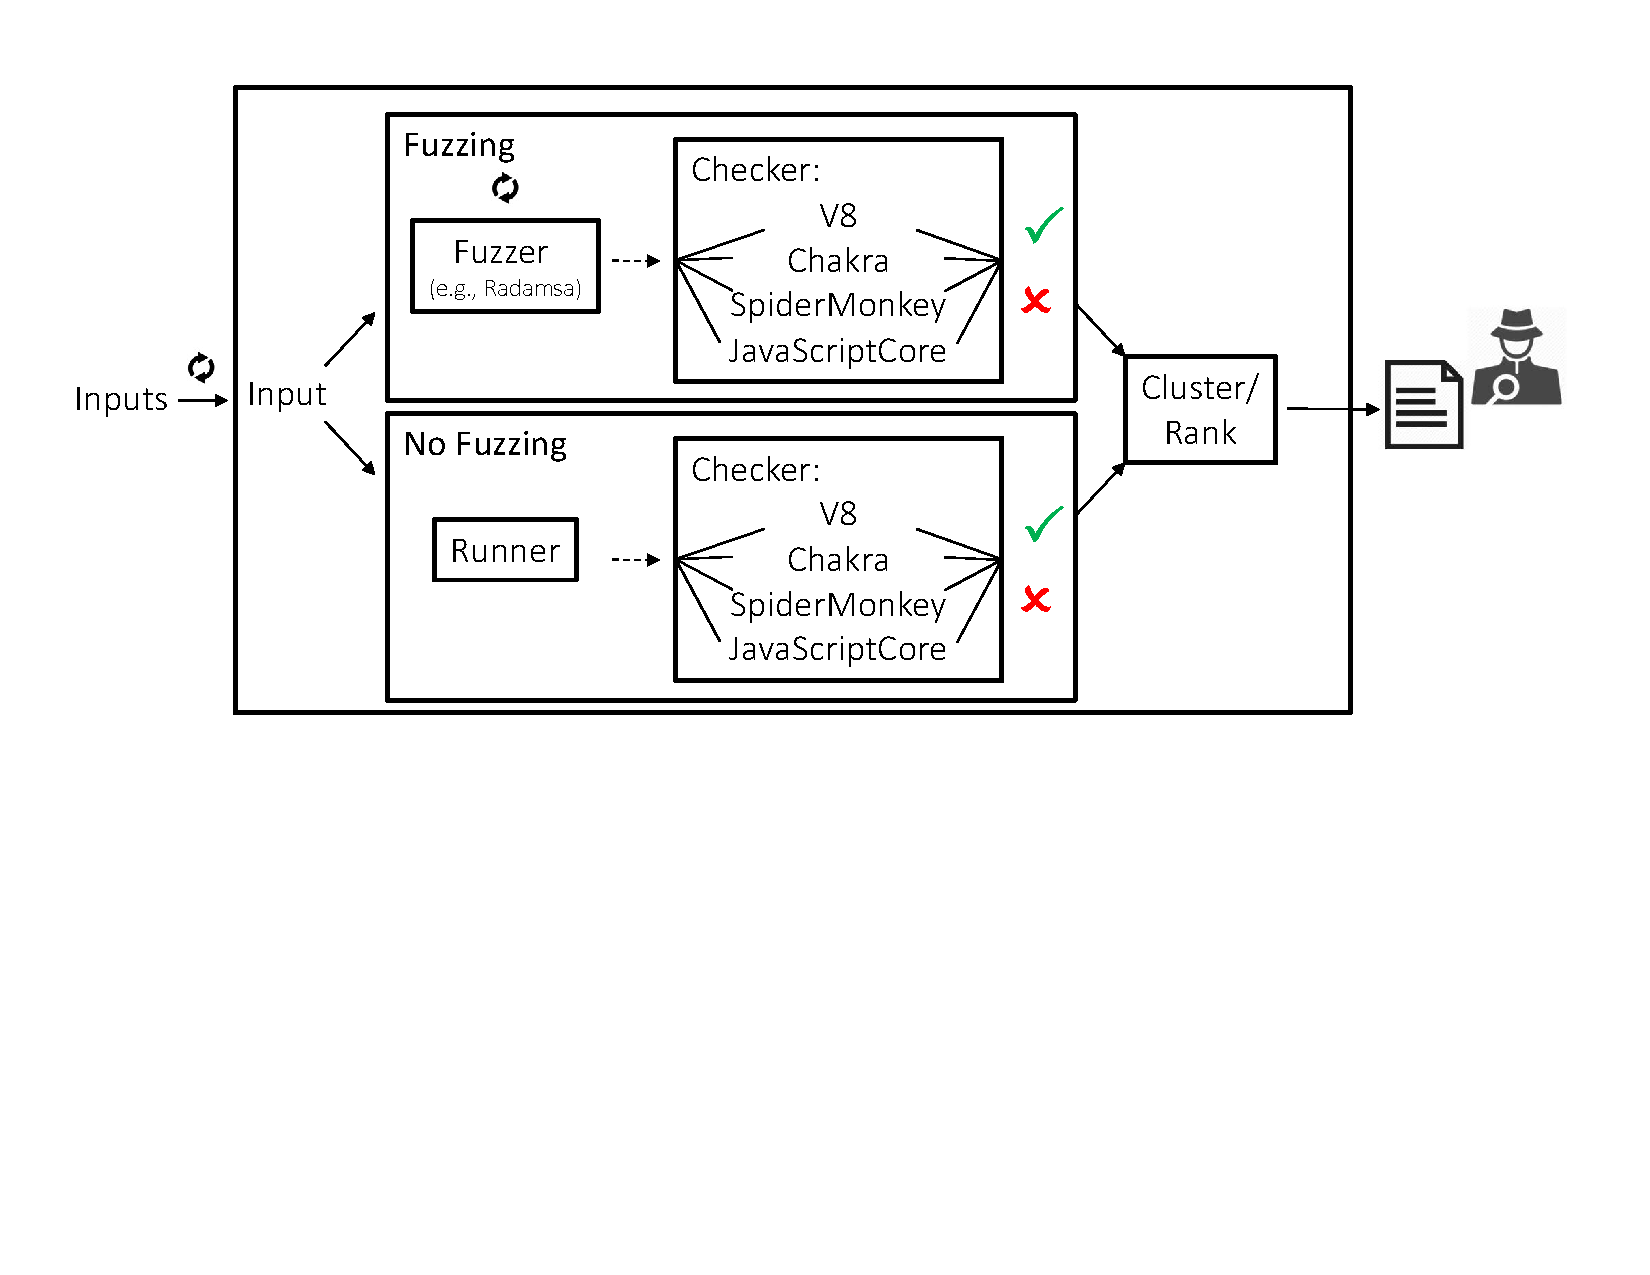
\includegraphics[trim=0 250 0 0,clip,width=0.5\textwidth]{google-awards-workflow}  
  \caption{\label{fig:workflow}Infrastructure.}
\end{figure}

Figure~\ref{fig:workflow} illustrates the workflow of the
infrastructure we used in this study. Boxes denote encapsulation;
arrowed lines indicate control flow (dashed) and data flow
(filled). The cycle icons denote repetition--the leftmost icon
indicates that each file in the input list will be analyzed in
separate whereas the rightmost icon indicates that a single file will be
processed multiple times in fuzzing mode. The bug-finding process
takes on input JS files from regression test suites of various JS
engines.

The bug-finding process works as follows.  Considering the case
fuzzing is not selected, as illustrated in the inner box at the bottom
of the figure, the oracle checks whether or not the output produced
for that file is consistent across all engine implementations. In case
the test passes in all engines or fails in all engines (\ie{}, the
output is consistent), the infrastructure discards the corresponding
input (mark ....). Otherwise, it considers the input as potentially
fault-revealing; hence interesting for human inspection. Considering
the case where fuzzing~\cite{fuzz-testing-history} is selected, new
inputs are obtained from a given input using some off-the-shelf
fuzzer\footnote{Several fuzzing methods have been proposed in the
  past, varying with respect to how new inputs are generated (\eg{},
  coverage-based~\cite{afl,honggfuzz},
  grammar-based~\cite{grammarinator,jsfunfuzz}, and
  random-based~\cite{radamsa}).}. The workflow is similar to that of
no fuzzing. In this case, however, multiple warnings can be produced
for a given seed input.

The infrastructure outputs a list of warnings for human inspection.
To reduce the number of false alarms, we clustered warnings in two
groups, reflecting their likelihood to manifest a real bug. The HI
group includes those inputs where execution manifests anomaly during
the execution of the test code or its close neighborhood\Comment{ as
  opposed to that of some internal JS function}. The rationale is that
the test in this group executed without violating any internal checks
of the API.  The LO group, in contrast, includes those cases where the
anomaly was observed during the execution of some API function. We
found that engine implementations often check pre-conditions of API
functions differently. It can happen, for example, that one engine
enforces a pre-condition that another engine does not. In those cases,
our infrastructure would observe a discrepancy that is more likely to
be associated with a bug in the (fuzzed) test; not the code. Although
we did find real bugs from warnings in the LO group, the proportion
was much lower compared to the HI group--only 12\% of the reals bugs
we found originated from the LO category. \Mar{show real examples of
  HI and LO and provide the rationale for such classification.}
\Mar{can we detect dups mining issue trackers?}

\begin{table*}[h!]
  \vspace{-3ex}
%  \scriptsize
  \centering
  \caption{List of bug reports issued by our team
    24, 2018.}
  \label{tab:bugs}
  \begin{tabular}{cccccccc}
    \toprule
    Issue\#    & Date & Fuzz & Engine  & Status  & \multicolumn{1}{c}{Url}  & Priority & Seed \\
    \midrule    
    1  & 4/12 & radamsa & Chakra   & \textbf{Fixed}  & \href{https://github.com/Microsoft/ChakraCore/issues/4978}{\#4978} & HI & webkit.jstests.es6 \\ 
    2  & 4/12 & radamsa & Chakra   & Rejected  & \href{https://github.com/Microsoft/ChakraCore/issues/4979}{\#4979} & HI & webkit.jstests.es6 \\
    3  & 4/14 & radamsa & JavascriptCore  & New & \href{https://bugs.webkit.org/show\_bug.cgi?id=184629}{\#184629}  & HI & webkit.jstests.es6    \\
    4  & 4/18 & \crossmark & JavascriptCore  & New  & \href{https://bugs.webkit.org/show\_bug.cgi?id=184749}{\#184749} & HI & JerryScriptjs.ecma      \\
    5  & 4/23 & \crossmark & Chakra  & \textbf{Confirmed}  & \href{https://github.com/Microsoft/ChakraCore/issues/5033}{\#5033} & HI & mozilla      \\
    6  & 4/25 & radamsa & Chakra  & \textbf{Fixed}     & \href{https://github.com/Microsoft/ChakraCore/issues/5038}{\#5038} & HI & JerryScriptjs.ecma   \\
    7  & 4/29 & \crossmark & Chakra  & \textbf{Confirmed}   &
    \href{https://github.com/Microsoft/ChakraCore/issues/5065}{\#5065} & HI & mozilla
    \\
    \midrule
    \multirow{2}{*}{8}  & \multirow{2}{*}{4/29} &  \multirow{2}{*}{\crossmark} & Chakra & \textbf{Confirmed} &    \href{https://github.com/Microsoft/ChakraCore/issues/5067}{\#5067} & \multirow{2}{*}{HI} & \multirow{2}{*}{mozilla}\\
                        &  &                       &
    JavascriptCore & New &    \href{https://bugs.webkit.org/show\_bug.cgi?id=185130}{\#185130}  &   & \\
    \midrule    
    9  & 4/29 & radamsa & JavascriptCore  & New  &    \href{https://bugs.webkit.org/show\_bug.cgi?id=185127}{\#185127}  & HI  & JerryScriptjs.ecma\\
    \midrule    
    \multirow{2}{*}{10} & \multirow{2}{*}{4/30}  & \multirow{2}{*}{radamsa} & Chakra & \textbf{Confirmed} &    \href{https://github.com/Microsoft/ChakraCore/issues/5076}{\#5076} & \multirow{2}{*}{HI} & \multirow{2}{*}{tinyjs.tests}\\    
                        &                        &        &
    JavascriptCore & New &
    \href{https://bugs.webkit.org/show\_bug.cgi?id=185156}{\#185156} &  & 
    \\
    \midrule    
    11 & 5/02 & radamsa & JavascriptCore  & New & \href{https://bugs.webkit.org/show\_bug.cgi?id=185197}{\#185197} & LO & mozilla \\
    12 & 5/02 & \crossmark & JavascriptCore & New  & \href{https://bugs.webkit.org/show\_bug.cgi?id=185208}{\#185208} & HI & mozilla \\
    13 & 5/10 & radamsa & Chakra & \textbf{Confirmed} & \href{https://github.com/Microsoft/ChakraCore/issues/5128}{\#5128} & HI & JerryScriptjs.regression \\
    14 & 5/17 & radamsa & Chakra & \textbf{Fixed} & \href{https://github.com/Microsoft/ChakraCore/issues/5182}{\#5182} & HI & v8.test.benchmarks\\
    15 & 5/17 & \crossmark & Chakra & \textbf{Confirmed} & \href{https://github.com/Microsoft/ChakraCore/issues/5187}{\#5187} & HI & webkit.jstests.es6\\
    16 & 5/21 & \crossmark & Chakra & \textbf{Confirmed} & \href{https://github.com/Microsoft/ChakraCore/issues/5203}{\#5203} & LO & mozilla\\
    17 & 5/24 & radamsa & JavascriptCore & New  & \href{https://bugs.webkit.org/show\_bug.cgi?id=185943}{\#185943} & HI & webkit.jstests.es6\\
    18 & 6/26 & radamsa & JavascriptCore & New  & \href{https://bugs.webkit.org/show_bug.cgi?id=187042}{\#187042} & HI & JerryScriptjs.regression\\
    19 & 6/28 & \crossmark & Chakra & Confirmed  & \href{https://github.com/Microsoft/ChakraCore/issues/5388}{\#5388} & HI & webkit.jstests.es6\\
   \bottomrule     
  \end{tabular}
\end{table*}


\section{Objects of Study}
\label{sec:methodology}

This section discusses the objects we used in our study.

%% methodology we used in our study.  The
%% dependent and independent variables will be discuss in
%% Section~\ref{sec:results}.

\subsection{Engines}
\label{sec:methodology:engines}~We selected the most popular JS
engines on the web~\Fix{cite} to focus our bug-finding efforts, namely
Microsoft's Chakra~\cite{chakra2018repo}, Google's
v8~\cite{v82018repo}, Mozilla's
SpiderMonkey~\cite{spidermonkey2018repo}, and Apple's JavaScriptCore
(WebKit)~\cite{jsc2018repo}.

\subsection{Seed JS files}~We considered in our study test suites
associated with all four JS engines we analyzed
(section~\ref{sec:methodology:engines}). In addition, we mined test
suites from other repositories based on the following criteria:
\begin{itemize}
  \item The project must be an open-source project and at least 1K stars from community.
  \item The repository must have JavaScript tests included.
  \item The tests should be plug-and-play and/or easy
    integration.\Mar{not clear what you mean}
\end{itemize}

Figure~\ref{fig:query} illustrates the Github API query\Fix{cite} we
used.\Mar{identify sources assoc. with the four analyzed engines.} The results of this query is sorted in descending order of
stars. Initially, we obtained a total of \Fix{XX} projects. Manually,
we follow the criteria to exclude invalid projects and we obtained a
total of \Fix{XX} repositories. Table~\ref{tab:test-suites} shows the
JS sources we considered. Overall, we found a total of \totfiles{} JS
files.\Mar{Briefly explain these names}

\begin{table}[h]
  \centering
  \caption{\label{tab:test-suites}Test Suites}
  \begin{tabular}{ccr}
    \toprule
    TestSuite & Source & \# JS files \\
    \midrule
    Duktape & \cite{duktape} & 997 \\
    JerryJS & \cite{jerryscript} & 1,803 \\
    JSI & \cite{jsi} & 99 \\
    Tiny-js & \cite{tinyjs} & 44 \\
    Mozilla & \Fix{??} & 32,414 \\
    V8.test.benchmarks.data & \Fix{??} & 64 \\
    WebKit.jstests.es6 & \Fix{??} & 605 \\
    WebKit.jstests.microbenchmarks & \Fix{??} & 426 \\
    \midrule
     &  & 36,452 \\
   \bottomrule     
  \end{tabular}
\end{table}

\begin{figure}
  \centering
  \begin{lstlisting}
https://api.github.com/search/repositories?q=javascript-engine+stars:>=1000&sort=stars
  \end{lstlisting}
  \caption{\label{fig:query}
  Query to the GitHub API for JS engines projects that contain over 1K stars.\Fix{fix query}
  }
\end{figure}

It is worth noting that many projects use distinct frameworks for
testing and require external libraries to run their testing
suites. For some projects, we made small changes in the testing
infrastructure to be able to uniformly run the test in all
engines.\Mar{not entirely clear what you did to support
  this.$\rightarrow$}We aimed to use only the JS file with minor fixes
to support our environment. These fixes are composed by an assertion
function that throws an Error that we can capture by our
infraestruture.

% For example to run the JerryScript tests it was necessary 
% use the unit-test package to run it, but with our changes we added the assertion
% does not have an assertion in the test file
% \Fix{add code to explain}

\subsection{Fuzzers}

\Mar{revise...}~We used representatives of popular fuzzing approaches. For
random-based fuzzing we used Radamsa~\cite{radamsa}; for
coverage-based fuzzing we used
\Fix{AFL~\cite{afl}/libfuzzer~\cite{libfuzzer}?}, and for
generative-based fuzzing we used
\Fix{grammarinator,jsfunfuzz?}. Details on how these fuzzers work can
be found elsewhere~\cite{fuzz-bart}.

Fuzzers grammar-based can generate a new file through a language grammar (ie. BNF).
Our infrastructure supports any grammar fuzzer with a few adjusts. However, 
we try to integrate several grammar-based fuzzers, for example 
Grammarinator~\footnote{https://github.com/renatahodovan/grammarinator}, QuickFuzz~\cite{grieco2016quickfuzz}
and \Fix{others fuzzers} to generate new JavaScript files based on grammar, but 
after several runs it was observed that this approach was ineffective
due the amount of invalid files and/or files without discrepancies. For example, if we ran 
Grammarinator to generate 1K JS files ten times with a random seed generation, we obtained
\Fix{XX\%} of valid files. Checking in our environment almost \Fix{XX\%}
are js files that shows undefined variables and due the differential testing in our environment
all engines will raise a SyntaxError and this approach was not relevant to our experiment.

\section{Bugs Found}
\label{sec:bugs}

%% Although there are many features yet to implement in our
%% infrastructure, 

This section shows results obtained with our
infrastructure. Table~\ref{tab:bugs} shows the list of bugs we
reported on issue trackers of different engines in the period of 42
days. So far, ten of the bugs we reported
were confirmed, two of which were fixed. One bug report we
submitted was rejected on the basis that the offending JS file
manifested an expected incompatibility across engine
implementations.
Note from the table that all bug
reports still waiting for confirmation are associated with the
JavaScriptCore engine (JSC). A closer look at the JSC issue tracker
showed that the triage process is very slow for that engine. As of
now, we did not find any new bug on SpiderMonkey and V8; the bugs we
found were duplicates and were not reported. Finally, it is
worth noting that 8 of the 19 JS files that manifested
discrepancies were \emph{not} produced with fuzzing (column
``Fuzz''). These are test files from suites of different engines. This
observation emphasizes the importance of continuously collecting test suites from
multiple sources; today, we use test suites from seven different open
source engines, including a total of 30K test files.

\Mar{justify why we discuss these bugs} \Mar{discuss other bugs}

\vspace{1ex}\noindent\textbf{Bug \# 6.} The JS code \CodeIn{var a = \{valueOf:~function()\{return
  ``\textbackslash{}x00''\}\} assert(+a === 0)\}} 
manifested a bug in the \js{} engine Chakra.  The object
property \CodeIn{valueOf} stores a function that returns a primitive
value identifying the target object~\cite{valueof}. The original
version of this code returns an empty string whereas the version of
the code modified by the Radamsa fuzzer~\cite{radamsa} returns a string
representation of a null character (called \CodeIn{NUL} in ascii). The
unary plus expression ``\CodeIn{+a}", appearing in the assertion, is
equivalent to the abstract operation \CodeIn{ToNumber(a.valueOf())}
that converts a string to a number, otherwise the operation returns
NaN (Not a Number)\cite{unary-plus}. For this case, Chakra evaluates
the unary plus to NaN as expected, as the null character cannot be
converted. As result, the test fails as expected. Chakra, in contrast,
incorrectly converts the string to zero, making the test to pass. All
other engines fail on this test. As Table~\ref{tab:bugs} shows, the
Chakra team fixed the issue soon after we reported the problem.

\section{Results}
\label{sec:results}

\Igor{
  In this section we discuss our findings to reach
  bugs in JS engines. Our experiments shows that fuzzing existents files
  still effective over the inputs without fuzzing.
}

\subsection{Dependent and Independent variables.}

The independent variable of our experiment is the fuzzing strategy as
implemented by various fuzzing tools. Our dependent variables are (i)
the ratio of bugs found with fuzzing versus no fuzzing and (ii) and
the ratio of bugs found with each fuzzing strategy. We consider a
search successful only if it lends in a bug confirmed by the
developers of the affected engine.  The rationale for considering the
ratio of bugs found with fuzzing versus no fuzzing is to observe how
often fuzzing really helps in this scenario. In the limit, all bugs
could be found without extra inputs, \ie{}, simply executing the seed
inputs on each engine and comparing their outcomes. Recall that we
mined test suites from a variety of sources. The rationale for
considering the fuzzing strategy is to understand to which extent each
strategy--as implemented by representative tools--helps in this
context.

\subsection{Fuzzing versus No Fuzzing}
\Fix{nao entendi muito sobre essa subsection... 
seria explicacao do porque utilizar o fuzzing baseado nos nosso resultados?}
\Igor{
  Os engines JS mais populares foram arduamente testados ao longo dos últimos anos, 
  o sistema robusto nao significa que esta livre de bugs, ao contrario,
  estamos testando-o com simples entradas a partir de testes de regressao 
  de bugs previamente encontrados, porem estas entradas poderiam servir como seeds 
  para novos testcases. Partindo disso, realizar fuzzer em arquivos 
  existentes em projetos open-sources eh uma maneira de
  aumentar ainda mais a eficiencia destes engines, por exemplo o Google incentiva o 
  uso de fuzzers no seu ecossistema\cite{oss-fuzz,honggfuzz}.
  
  Nosso estudo revelou que dos \Fix{19} bugs reportados pelo nosso time, 
  apenas 8 nao foram fuzzados \Fix{42.1\%}, isso se da 
  a importancia tanto de utilizar fuzzing em arquivos de teste do proprio projeto,
  quanto em projetos distintos de mesma ordem, pois neste caso engines JS 
  devem interpretar arquivos, entao quanto mais entradas, melhores os resultados.
  \Fix{discuss}
}

\subsection{Fuzzing Strategy}
\Igor{
  Para realizar nossos experimentos, tivemos que decidir qual as 
  melhores abordagens para aumentar a efetividade dos fuzzers.
  Os fuzzers mutacionais se mostraram mais eficientes em relacao
  aos fuzzers geracionais, entao focamos neste ponto.
  Utilizamos os fuzzers radamsa, QuickFuzz e \Fix{others} nas suas configuracoes
  default para realizar a mutacao em arquivos existentes.
  O fuzzer radamsa eh um fuzzer mutacional agnostico de linguagem e possui algumas
  deficiencias para a nossa infraestrutura como a falta de uma gramatica para guiar a suas mutacoes, 
  pois muitas das vezes a unica mutacao ocorre em uma palavra dentro de um comentario por exemplo.
  O fuzzer QuickFuzz tem uma gramatica JS integrada e sua mutacao ocorre de forma mais robusta que o 
  radamsa, gerando arquivos mais relevantes.
  Nossa infraestrutura usa a library Esprima\footnote{cite esprima url} para garantir que o arquivo fuzzado
  é um arquivo de teste relevante, seguindo estes requisitos:
  \begin{itemize}
    \item it contains only unicode text
    \item it is parseable (i.e., it is structurally well-formed)
    \item it does not contain engine-specific functions  
    \item it does not empty
  \end{itemize}

}

\section{Related Work}

RFC-Directed Differential Testing of Certificate Validation in SSL/TLS Implementations...[ICSE18]

%\section*{Acknowledgment}

%\bibliographystyle{IEEEtran}
\bibliographystyle{plain}
\bibliography{references,../docs/google-research-awards-latam/tmp}

\end{document}
